\section{Results}
\label{sec:results}

\subsection{Quality--opportunity paths differ by intervention and scale}

Figure~\ref{fig:absolute} shows all 90 evaluated points.  The post-hoc A0 and
A1-H paths initially buy opportunity at modest loss cost, then exit the plotted
loss range as clipping approaches .9.  The trained paths occupy different
regions: their gates create substantial exact zeros already at $\kappa=0$,
while higher thresholds move them farther right.  No one family dominates the
entire evaluated set.

The endpoint ordering is consistent at high dose.  At $\kappa=.5$, \Aseven{}
has both lower loss and higher $\Rmodel$ than \Afour{} at every scale
(Table~\ref{tab:cross-scale-endpoints}).  Its opportunity advantage is large:
14.8, 5.0, and 9.0 percentage points at 14M, 70M, and 410M.  At
$\kappa=0$, by contrast, \Afour{} is better on both axes at 14M and 70M,
whereas \Aseven{} is better at 410M.  Thus the high-dose ordering replicates
descriptively across the three cohorts; the zero-threshold ordering does not.

% Generated by analyses/012-2026-09-04-paper-synthesis/01_build.py
\begin{table}[t]
\centering
\caption{Low- and high-dose trained endpoints. Each cell is validation loss / $R_{model}$ (\%). A4-OL1 and A7-OL1 are complete recipes, not an isolated topology contrast.}
\label{tab:cross-scale-endpoints}
\small
\begin{tabular}{lrrrr}
\toprule
& \multicolumn{2}{c}{A4-OL1} & \multicolumn{2}{c}{A7-OL1} \\
\cmidrule(lr){2-3}\cmidrule(l){4-5}
Model & $\kappa=0$ & $\kappa=.5$ & $\kappa=0$ & $\kappa=.5$ \\
\midrule
14M & 5.458 / 7.8 & 6.038 / 12.7 & 5.480 / 7.1 & 5.829 / 27.5 \\
70M & 4.805 / 25.7 & 5.389 / 35.6 & 4.941 / 23.6 & 5.216 / 40.6 \\
410M & 5.692 / 38.3 & 5.191 / 71.6 & 5.426 / 41.1 & 5.121 / 80.6 \\
\bottomrule
\end{tabular}
\end{table}


\subsection{Local zero mass does not determine model-wide opportunity}

Figure~\ref{fig:sites} resolves the low- and high-dose endpoints by activation
site.  One-sided gates yield broad exact-zero mass at $a,m,h,z$ even when
$\kappa=0$.  At $\kappa=.5$, \Afour{} drives $h$ and $z$ to essentially 100\%
zeros, but leaves $q,k,v$ dense.  \Aseven{} instead creates large exact-zero
mass throughout attention.  Its high-dose $(q,k,v)$ rates are
$(93.5,94.5,98.7)$\% at 14M, $(71.5,72.1,86.9)$\% at 70M, and
$(77.8,80.6,94.0)$\% at 410M.  This non-monotone cross-scale pattern already
argues against a scalar ``sparsity level'' as the full explanation.

\begin{figure*}[t]
  \centering
  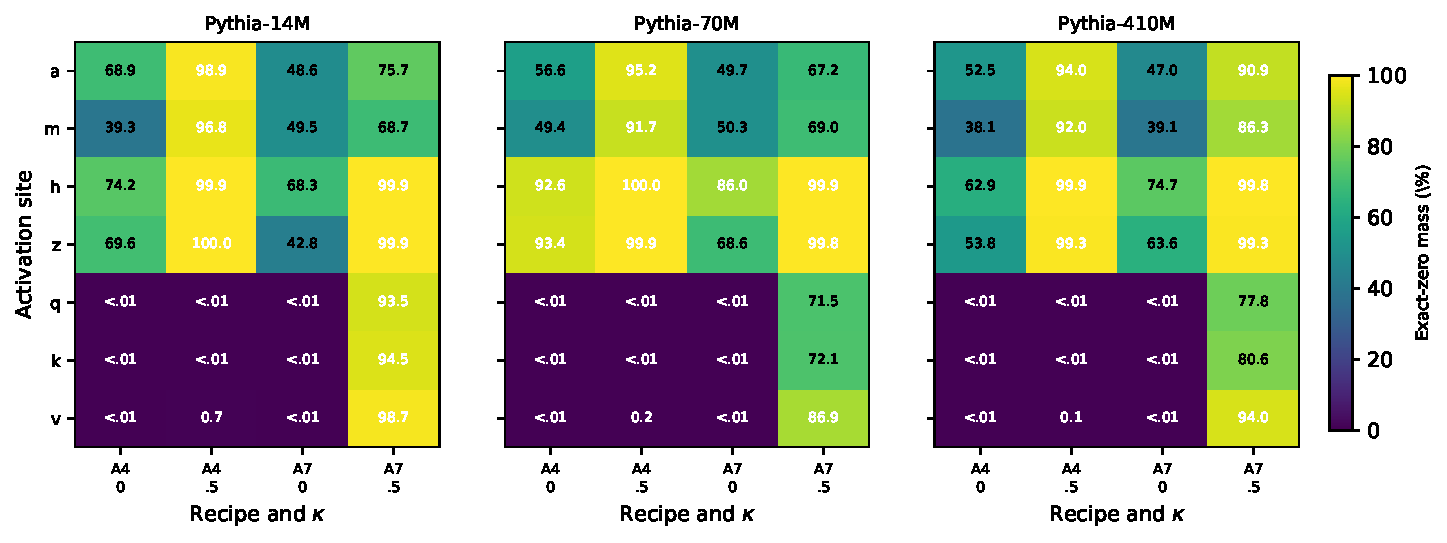
\includegraphics[width=.98\textwidth]{figures/03-sitewise-zero-structure.pdf}
  \caption{Integer-pooled exact-zero mass at seven activation sites for the
  trained low- and high-dose endpoints.  $q$ and $k$ are measured after RoPE;
  columns are complete recipes.  Values below .01\% are printed as $<.01$.}
  \label{fig:sites}
\end{figure*}

The operation decomposition in Figure~\ref{fig:operations} turns this local
structure into its graph-level consequence.  At 410M/$\kappa=.5$, \Afour{}
has \emph{more} zero mass than \Aseven{} at $a$ (94.0 vs. 90.9\%) and $m$
(92.0 vs. 86.3\%), yet \Aseven{} has higher $\Rmodel$ (80.6 vs. 71.6\%).
QK and PV contribute 11.1 percentage points available only to the seven-site
recipe, overcoming its local deficit.  Their combined contributions are 16.8,
10.4, and 11.1 points at 14M, 70M, and 410M.  This is a direct example of
topology and operand reuse changing a model-wide conclusion.

\begin{figure*}[t]
  \centering
  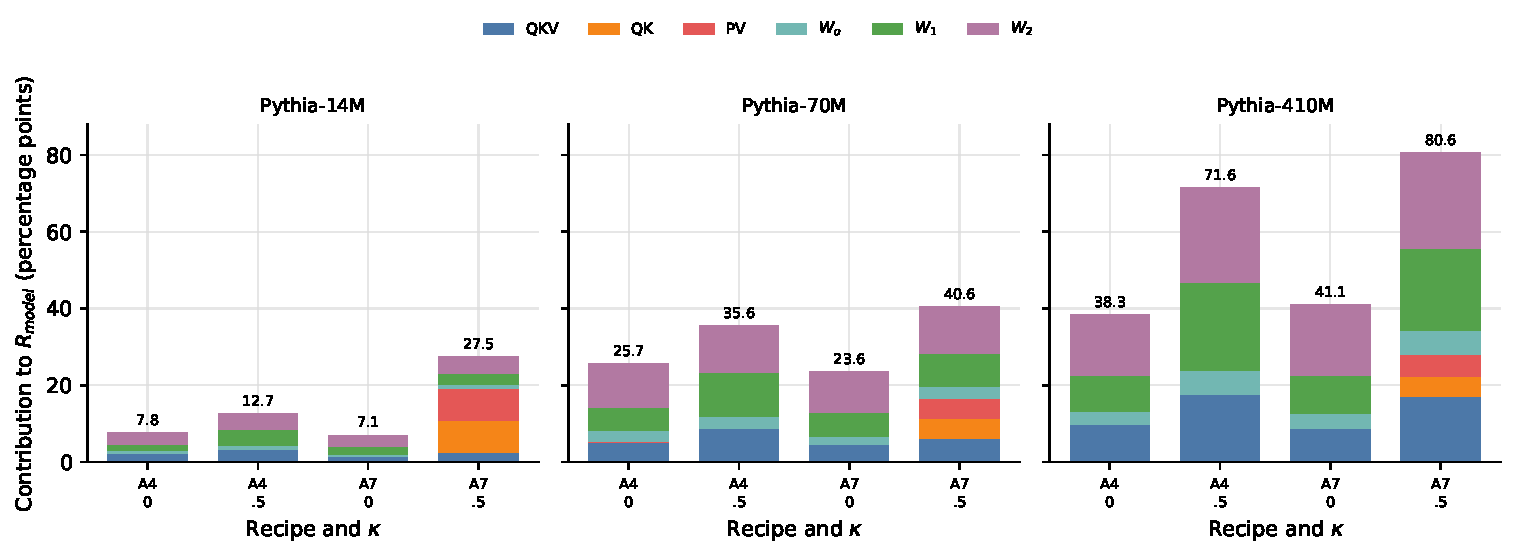
\includegraphics[width=.98\textwidth]{figures/04-operation-contributions.pdf}
  \caption{Contribution of each measured operation to $\Rmodel$ at trained
  endpoints.  Segment heights use the common model denominator, so each stack
  sums to the labeled total.  QK and PV use only valid causal positions.}
  \label{fig:operations}
\end{figure*}

\subsection{The 410M cohort is a boundary result}
\label{sec:410boundary}

Within both trained 410M recipes, raising $\kappa$ from 0 to .5 moves down and
right: \Afour{} changes by $-0.501$ loss and $+33.25$ opportunity points;
\Aseven{} by $-0.306$ and $+39.49$ points.  At 14M and 70M the corresponding
loss changes are positive: $+0.580/+0.584$ for \Afour{} and
$+0.349/+0.275$ for \Aseven{}.  This is not a claim that high-dose sparse 410M
beats its dense control---it does not.  It is a reversal \emph{within the
trained threshold ladders}.  The post-hoc paths at 410M continue to worsen
monotonically, separating an effect of training with the gates from robustness
to evaluation-only deletion (Appendix Figure~\ref{fig:deltas}).

The shared-token design makes a scale-only interpretation untenable.  Although
410M has six times the parameters of 70M, it receives the same tokens and only
3.7 tokens per parameter.  Its A0 validation loss (4.547) is worse than 70M
(4.100), it clips the global task gradient at 56 rather than 8 of 712
boundaries, and its maximum pre-clip norm is 26.96 rather than 3.51.  These raw
norms are not parameter-normalized, but they document a materially different
optimization trajectory.  A predeclared learning-rate screen selects the
original $3\times10^{-4}$ arm: mean late training loss is 4.494 at that rate,
4.513 at $6\times10^{-4}$, and 6.851 at $10^{-3}$; validation losses are 4.547,
4.552, and 6.787.  The grid therefore rejects a simple upward-LR repair, while
leaving training horizon unresolved.

